\chapter{Methodology}

This chapter introduces the tools, software, and methodology used to convert Genenetwork2's SQL tables to RDF.  To achieve the first and third objectives, which involve improving accessibility, interoperability, and interpretability of biological metadata, a Domain Specific Language (DSL) capable of converting SQL to RDF will be designed.  This DSL will enable an evaluation of the current limitations of the Genenetwork2 SQL database and an assessment of the benefits and drawbacks of migrating to RDF.  The second objective, which pertains to reviewing previous research on the GN platform, has already been addressed in the literature review.  Finally, to achieve the last objective, the performance of RDF in the context of Genenetwork2 will be compared to that of SQL.

\section{Tools and Software Used}

For this dissertation, the following tools and software will be used:

\begin{enumerate}
\item \textit{GNU/Linux}:  MacOS and Windows are not factored in at all in the development environment.  A GNU/Linux distribution is used because it is free, open and in wide usage for software development and deployment purposes.  MacOS and Windows are expensive.
\item \textit{GNU Guix} (\url{https://guix.gnu.org/}): This will act as a package manager to declaratively specify and control the dependencies for the dissertation, and guarantee bit for bit reproducibility.
\item \textit{GNU Guile} (\url{https://www.gnu.org/software/guile/}): GNU Guile, as a dialect of Scheme, will be the primary programming language utilized to develop the SQL to RDF parser. Its robust macro system will facilitate the creation of a declarative and expressive Domain Specific Language that will greatly aid in parsing SQL to RDF.
\item \textit{MariaDB} (\url{https://mariadb.org/}): This is an open-source RDBMS that is a fork of MySQL which can be used as a drop-in replacement for MySQL.  MariaDB will primarily be used as the SQL data source in this dissertation.
\item \textit{Virtuoso} (\url{https://virtuoso.openlinksw.com/}): This is an open source high-performance engine that can be use to manage and query large amounts of RDF data.
\item \textit{Graphviz} (\url{https://graphviz.org/}): This is an open-source graph visualization software that is used to visualize different types of graphs.
\item \textit{rapper} (\url{https://librdf.org/raptor/rapper.html}): This is a RDF parsing and serializing utility that can be used to lint RDF files that use the Turtle syntax.
\item \textit{pytorch} (\url{https://pytorch.org/}) or \textit{GPT-3} (\url{https://github.com/openai/gpt-3}): We will use a machine learning tool to scope AI needs. pytorch is a good candidate.  We will also try natural language processing, such as offered by GPT-3 and feed RDF to see what type of questions we can ask and provide future recommendations.
\end{enumerate}

\section{Data Collection}

The GN small database, a publicly accessible and reduced version of the main database, will be used as the primary source of data during the implementation of this dissertation.  The main database, which is constantly growing, hosted at the University of Tennessee Health Science Center, will be used to test and validate the results.  Testing and validation of the results will be done against the main database which is hosted at the University of Tennessee Health Science Center.

In addition to the Genenetwork2 database, other relevant datasets from external sources may also be collected and included in the analysis.  These sources may include publicly available biological databases, such as the Gene Ontology database or the Uniprot protein database.  Careful consideration will be given to the selection of these external datasets to ensure that they are relevant and reliable.

Overall, the data collection process for this dissertation will involve extracting the data from the Genenetwork2 database and potentially including additional relevant datasets from external sources.

\section{Design and Implementation}

The proposed parser will be a Domain Specific Language (DSL) that can transform SQL query results into valid RDF triples.  It will be a flexible database-agnostic parser that supports s-expressions.  This parser will declaratively describe how the results of a SQL query maps onto a pre-defined ontology.  Figure \ref{fig:parser-demo} shows how this parser would work.

\begin{figure}[H]
  \centering
  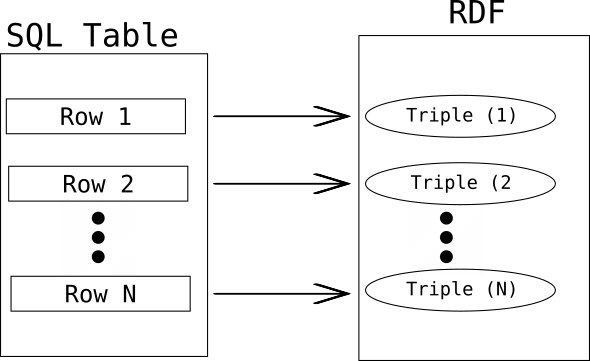
\includegraphics[width=8cm]{parserDemo}
  \caption{\textit{The parser operates on each row to produce a valid triple store}}
  \label{fig:parser-demo}
  \centering
\end{figure}

In order to support s-expressions, a special form is necessary to query SQL, especially when the structure of the table is not known.  To achieve this, a core set of macros will be designed to form the basis of the DSL.  The architecture design for the parser will primarily focus on functional requirements, specifically on creating a DSL that is user-friendly and naturally describes the process of converting table records into RDF subject-predicate-object triples.

\section{Development Methodology}

The development of a functional parser is a critical aspect of using RDF triple stores as the underlying data storage system for Genenetwork2's metadata in this dissertation. To achieve this, a \textit{rapid application development} methodology will be adopted, which involves minimal planning and rapid prototyping. This methodology is well-suited for Read-Eval-Print-Loop (REPL) driven development that is commonly used in the Lisp community.

With rapid prototyping, a working Domain Specific Language (DSL) will be created. Subsequently, the relevant tables will be parsed, and their performance will be evaluated in tandem. This approach will facilitate the incorporation of changes within the development, validation, and testing cycle, as heavy pre-planning is not required.

\section{Validation and Testing}

\subsection{Validation}

In order to validate the benefits and challenges of the ported Genenetwork2 database in RDF, a subset of the functionality provided by Genenetwork2, which is currently based on SQL, will be replaced with RDF.  This will enable a direct comparison of the speed and complexity of RDF versus SQL.  By measuring the time and resources required to perform specific tasks, we will be able to gain a deeper understanding of the trade-offs involved in using RDF, and how it compares to SQL in terms of data interoperability, integration, and scalability.

\subsection{Testing}

The first step in testing the output of the SQL to RDF parser involves utilizing \textit{rapper}, an RDF linter, to assess the accuracy of the RDF format.  This process, known as linting, ensures that the output is error-free, allowing the data to be ingested into RDF.  If no errors are detected during the linting process, the data can then be uploaded to a running Virtuoso instance.

Beyond linting, a subset of functionality in Genenetwork2 that uses SQL will be substituted with RDF with the expectation that there will be no loss in functionality.  This will be accompanied by integration tests and unit tests to ensure that the expected level of functionality is maintained.

\section{Expected Results}
The expected results are:

\begin{enumerate}

\item Faster and more efficient metadata access with RDF compared to SQL due to a better and more fluent representation of metadata.

\item The creation of an Embedded Domain Specific Language that generates RDF triples from SQL.

\item Seamless integration of the RDF data store with external resources such as UniProt (\url{https://www.uniprot.org/}).
\end{enumerate}
